\section{Diseño del modelo lógico y físico de datos del sistema}
    \subsection{Modelo relacional}
        \begin{figure}[H]
            \centering
            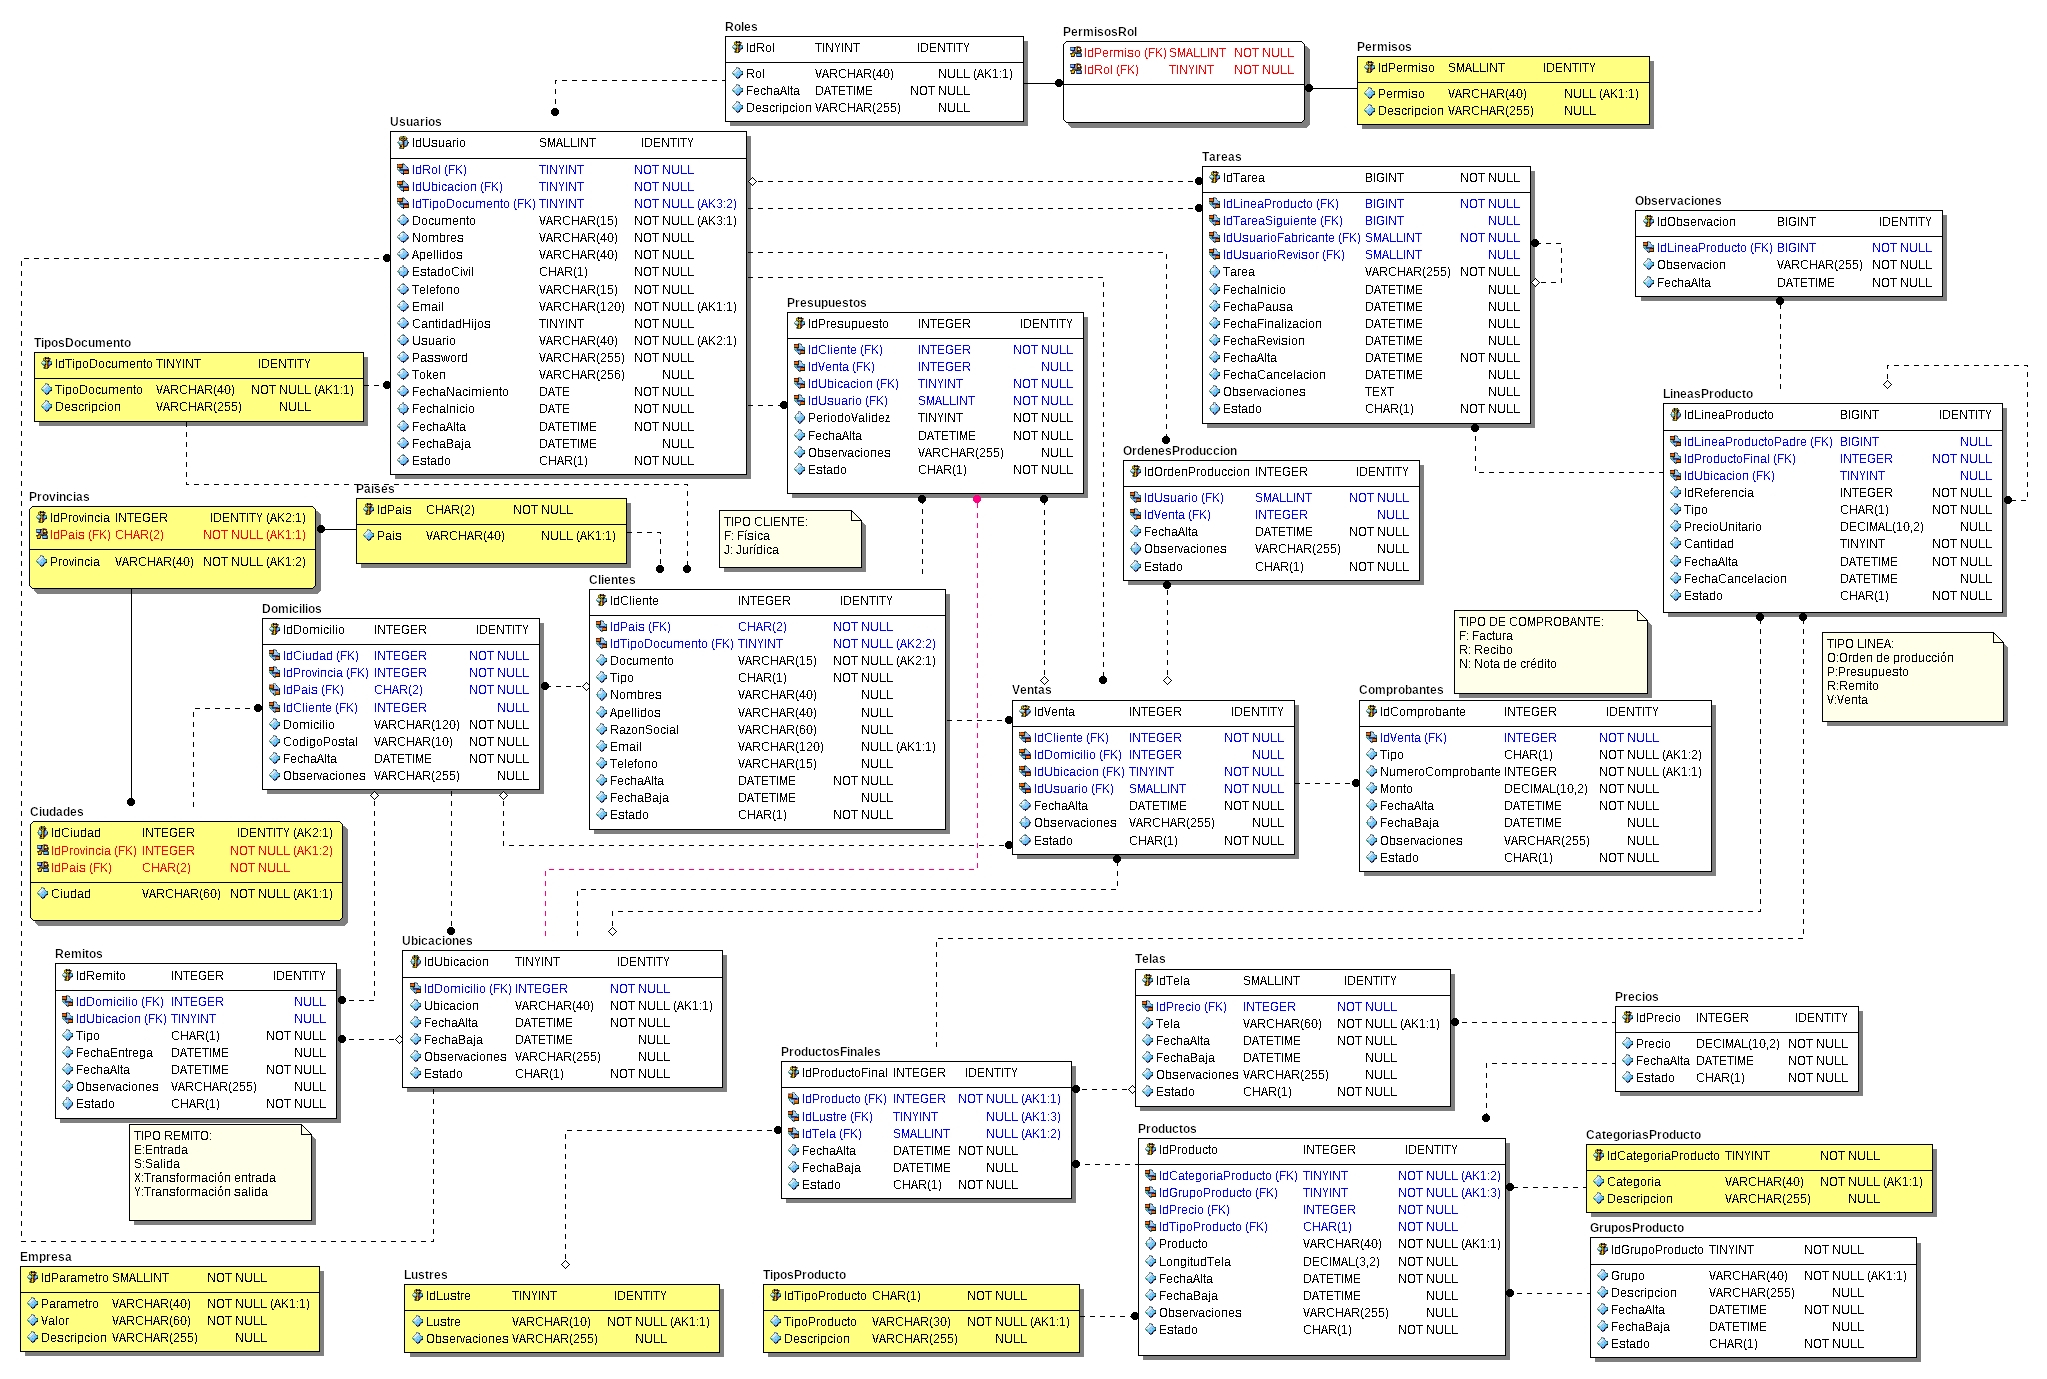
\includegraphics[width=\textwidth,height=\textheight,keepaspectratio]{ModeloRelacional/modeloRelacional}
            \caption{Modelo relacional}
        \label{fig:Modelo relacional}
        \end{figure}
        \clearpage %salto de pagina
        \begin{figure}[H]
            \centering
            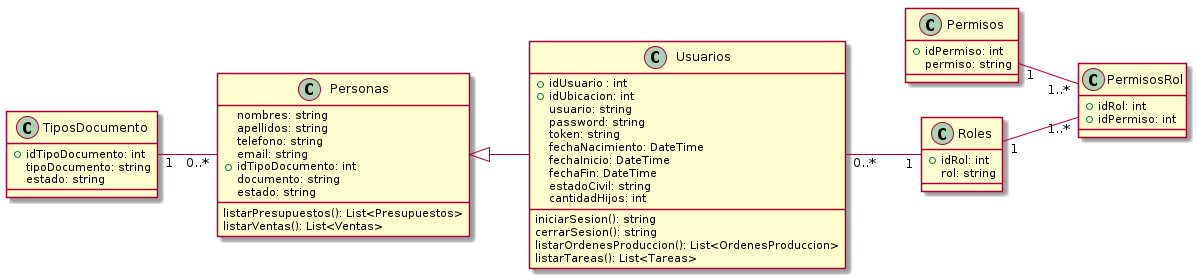
\includegraphics[width=\textwidth,height=0.90\textheight,keepaspectratio]{ModeloRelacional/vistaSistema}
            \caption{Modelo relacional - Vista sistema}
        \label{fig:Modelo relacional - Vista sistema}
        \end{figure}
        \begin{figure}[H]
            \centering
            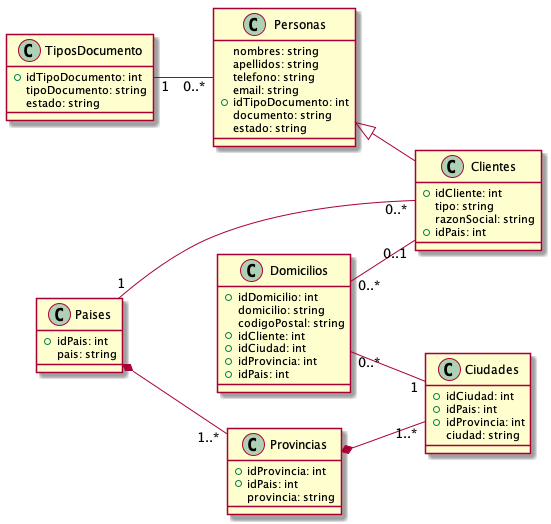
\includegraphics[width=\textwidth,height=0.90\textheight,keepaspectratio]{ModeloRelacional/vistaClientes}
            \caption{Modelo relacional - Vista clientes}
        \label{fig:Modelo relacional - Vista clientes}
        \end{figure}
        \begin{figure}[H]
            \centering
            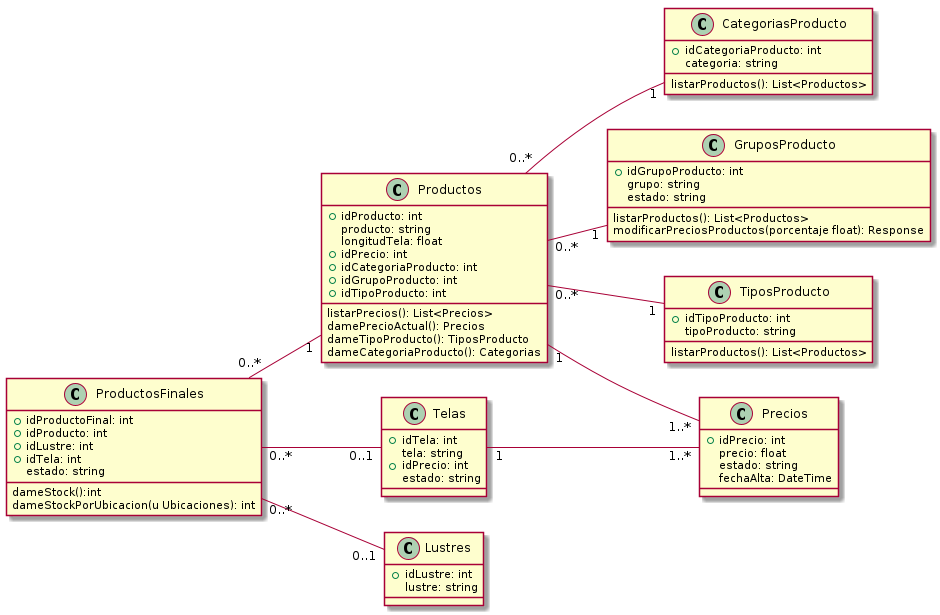
\includegraphics[width=\textwidth,height=0.90\textheight,keepaspectratio]{ModeloRelacional/vistaProductos}
            \caption{Modelo relacional - Vista productos}
        \label{fig:Modelo relacional - Vista productos}
        \end{figure}
        \begin{figure}[H]
            \centering
            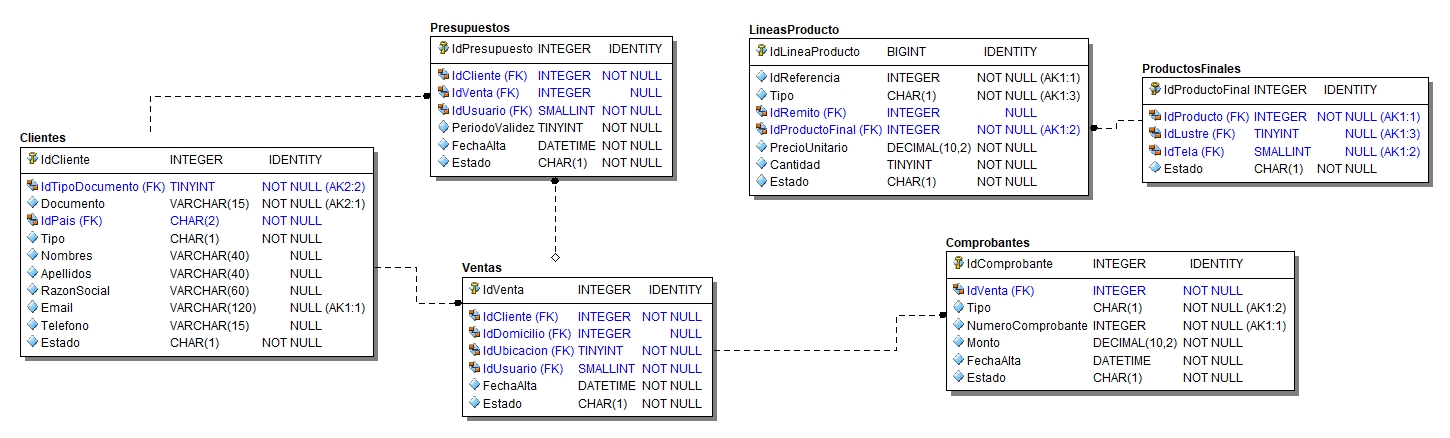
\includegraphics[width=\textwidth,height=0.90\textheight,keepaspectratio]{ModeloRelacional/vistaPresupuestosVentas}
            \caption{Modelo relacional - Vista presupuestos y ventas}
        \label{fig:Modelo relacional - Vista presupuestos y ventas}
        \end{figure}
        \begin{figure}[H]
            \centering
            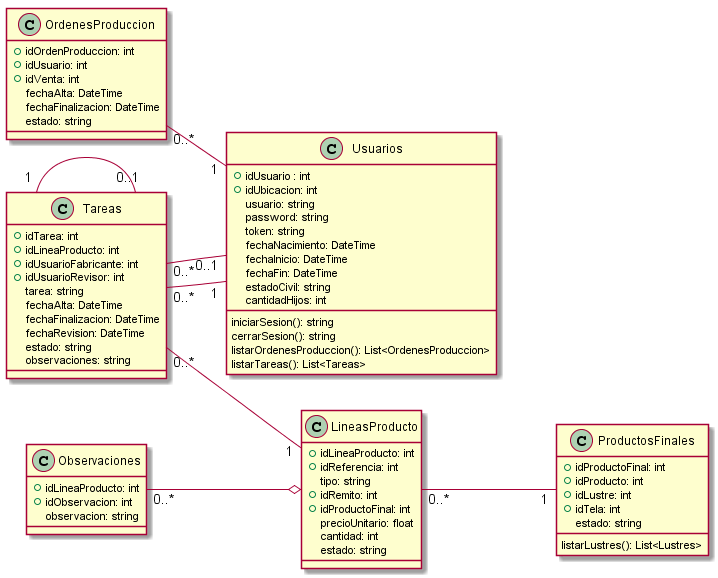
\includegraphics[width=\textwidth,height=0.90\textheight,keepaspectratio]{ModeloRelacional/vistaProduccion}
            \caption{Modelo relacional - Vista producción}
        \label{fig:Modelo relacional - Vista producción}
        \end{figure}

        \begin{figure}[H]
            \centering
            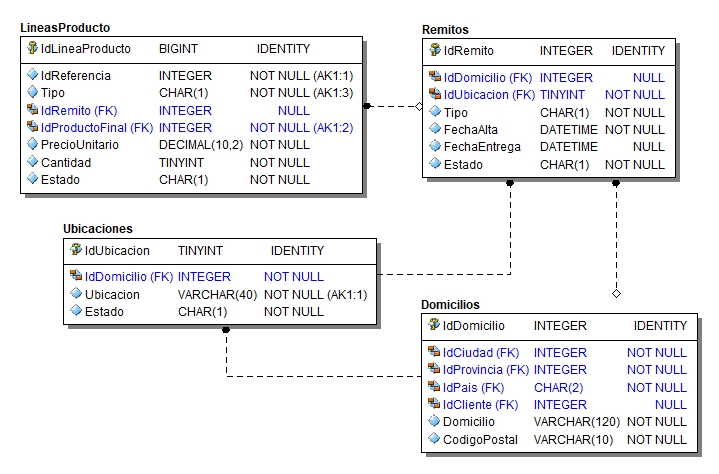
\includegraphics[width=0.7\textwidth,height=0.5\textheight,keepaspectratio]{ModeloRelacional/vistaEntregas}
            \caption{Modelo relacional - Vista entregas}
        \label{fig:Modelo relacional - Vista entregas}
        \end{figure}